\chapter{Aplicación web para el diagnóstico del Alzheimer mediante MRI}
\label{ch:aplicacion-web-para-el-diagnostico-del-alzheimer-mediante-mri}
Como segundo objetivo de este proyecto se plantea poder aplicar el estudio realizado en un ejemplo real, en este caso
en una aplicación web.
En este capítulo se detalla el proceso que se ha seguido hasta completarla.
Siguiendo la metodología comentada en el apartado~\ref{sec:metodologia-herramientas-y-obstaculos}.

\section{Especificación del sistema}\label{sec:especificacion-del-sistema}
Para poder completar una especificación del sistema es necesario conocer las necesidades de los usuarios, por lo que se
han creado 2 usuarios ficticios que darán forma a la HU que detalla el sistema.

\subsection{Usuarios}\label{subsec:usuarios}
\begin{table}[H]
    \centering
    \begin{tabular}{| l | l|}
        \hline
        Nombre & Blanca \\
        \hline
        Edad & 22 años \\
        \hline
        Ocupación & Estudiante de radiología \\
        \hline
        Personalidad & Extrovertida y analítica \\
        \hline
        Metas & Conseguir especializarse en el campo de radiología \\
        \hline
        Habilidades tecnológicas & Altas \\
        \hline
    \end{tabular}
    \caption{Usuarios ficticios: Persona 1}
    \label{tab:persona1}
\end{table}

\begin{table}[H]
    \centering
    \begin{tabular}{| l | l|}
        \hline
        Nombre & Ana \\
        \hline
        Edad & 45 años \\
        \hline
        Ocupación & Experta en radiología \\
        \hline
        Personalidad & Sensible y positiva \\
        \hline
        Metas & Poder mejorar el área de radiología del centro en el que trabaja \\
        \hline
        Habilidades tecnológicas & Altas \\
        \hline
    \end{tabular}
    \caption{Usuarios ficticios: Persona 2}
    \label{tab:persona2}
\end{table}


Blanca y Ana tienen un alto conocimiento teórico en este ámbito, forman parte de este estudio que se está realizando,
son futuras usuarias de la aplicación y participan como clientes de la misma realizando la historia de usuario que
define la especificación del sistema.

\subsection{Historia de Usuario}\label{subsec:historia-de-usuario}
La HU que se define es la siguiente:

\textbf{Como profesional de entornos clínicos quiero poder conocer el grado de Enfermedad de Alzheimer en una resonancia
magnética de manera sencilla.}

\begin{itemize}
    \item \textbf{Descripción}: Como usuario, quiero poder conocer cuál es el grado de enfermedad de Alzheimer presente
    en una neuroimagen, en concreto en una MRI de tipo \textit{NIfTI}.
    Con el objetivo de realizar un diagnóstico de enfermedad de Alzheimer sin necesidad de instalar ningún programa
    software para visualizar imágenes cerebrales
    \item \textbf{Pruebas de Aceptación del Usuario}: Subir un archivo \textit{NIfTI} y obtener una clasificación de la
    imagen y el valor del grado presente correspondiente en términos de Enfermedad de Alzheimer.

\end{itemize}

De esta necesidad surge \textbf{Alz Care}.

\textbf{Alz Care} se idea para ser una aplicación que una Inteligencia Artificial y salud.
En ella a partir de Imágenes por resonancia magnética se obtiene una clasificación del deterioro cognitivo y EA presentes.


\section{Proceso de Diseño}\label{sec:proceso-de-diseno}
En esta sección se muestra el proceso de diseño llevado a cabo para \textbf{Alz Care}, así como su identidad visual y
prototipos.

\subsection{Identidad visual}\label{subsec:identidad-visual}

\subsubsection{Paleta de colores}

La paleta de colores elegida es la siguiente:

\begin{figure}[H]
    \centering
    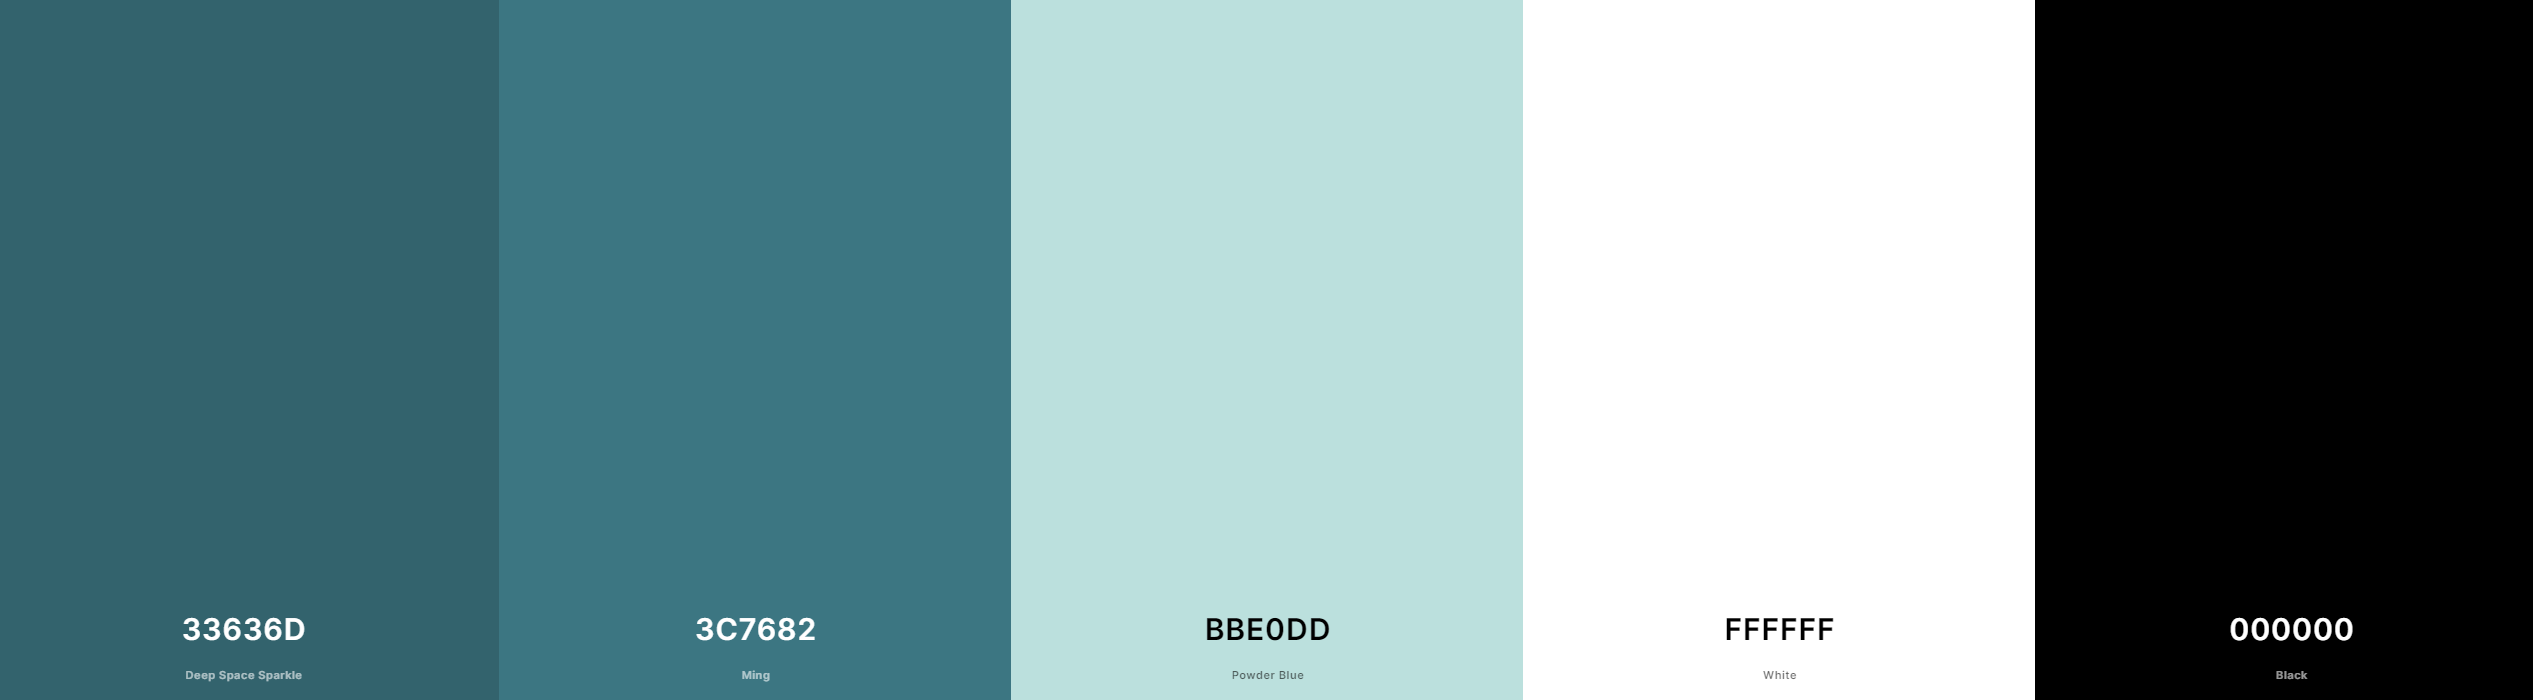
\includegraphics[width=0.6\textwidth]{./imgs/app/paleta}
    \caption{Paleta de colores de Alz Care}
    \label{fig:paleta-colores}
\end{figure}

Se elige esta paleta porque se busca minimalismo y serenidad y el uso de tonos verdes azulados para mantener una
relación con el mundo de la salud.

\subsubsection{Logotipo}

El logotipo de la aplicación se ha realizado usando la herramienta
Paint3D~\footnote{\href{https://apps.microsoft.com/store/detail/paint-3d/9NBLGGH5FV99?hl=es-es&gl=es}{Paint3D}}.

\begin{figure}[H]
    \centering
    
\includegraphics[width=\textwidth]{./imgs/app/icon-name}
    \caption{Logotipo de Alz Care}
    \label{fig:logotipo}
\end{figure}

\subsection{Mockup: UI UX Design}\label{subsec:mockup:-ui-ux-design}
Para facilitar el desarrollo de la misma, se ha realizado un prototipo de las páginas principales.
Se ha hecho uso de Figma~\footnote{\href{https://www.figma.com/}{Figma}} como herramienta de generación de prototipos.
Las vistas generadas son las siguientes:

\begin{figure}[H]
    \centering
    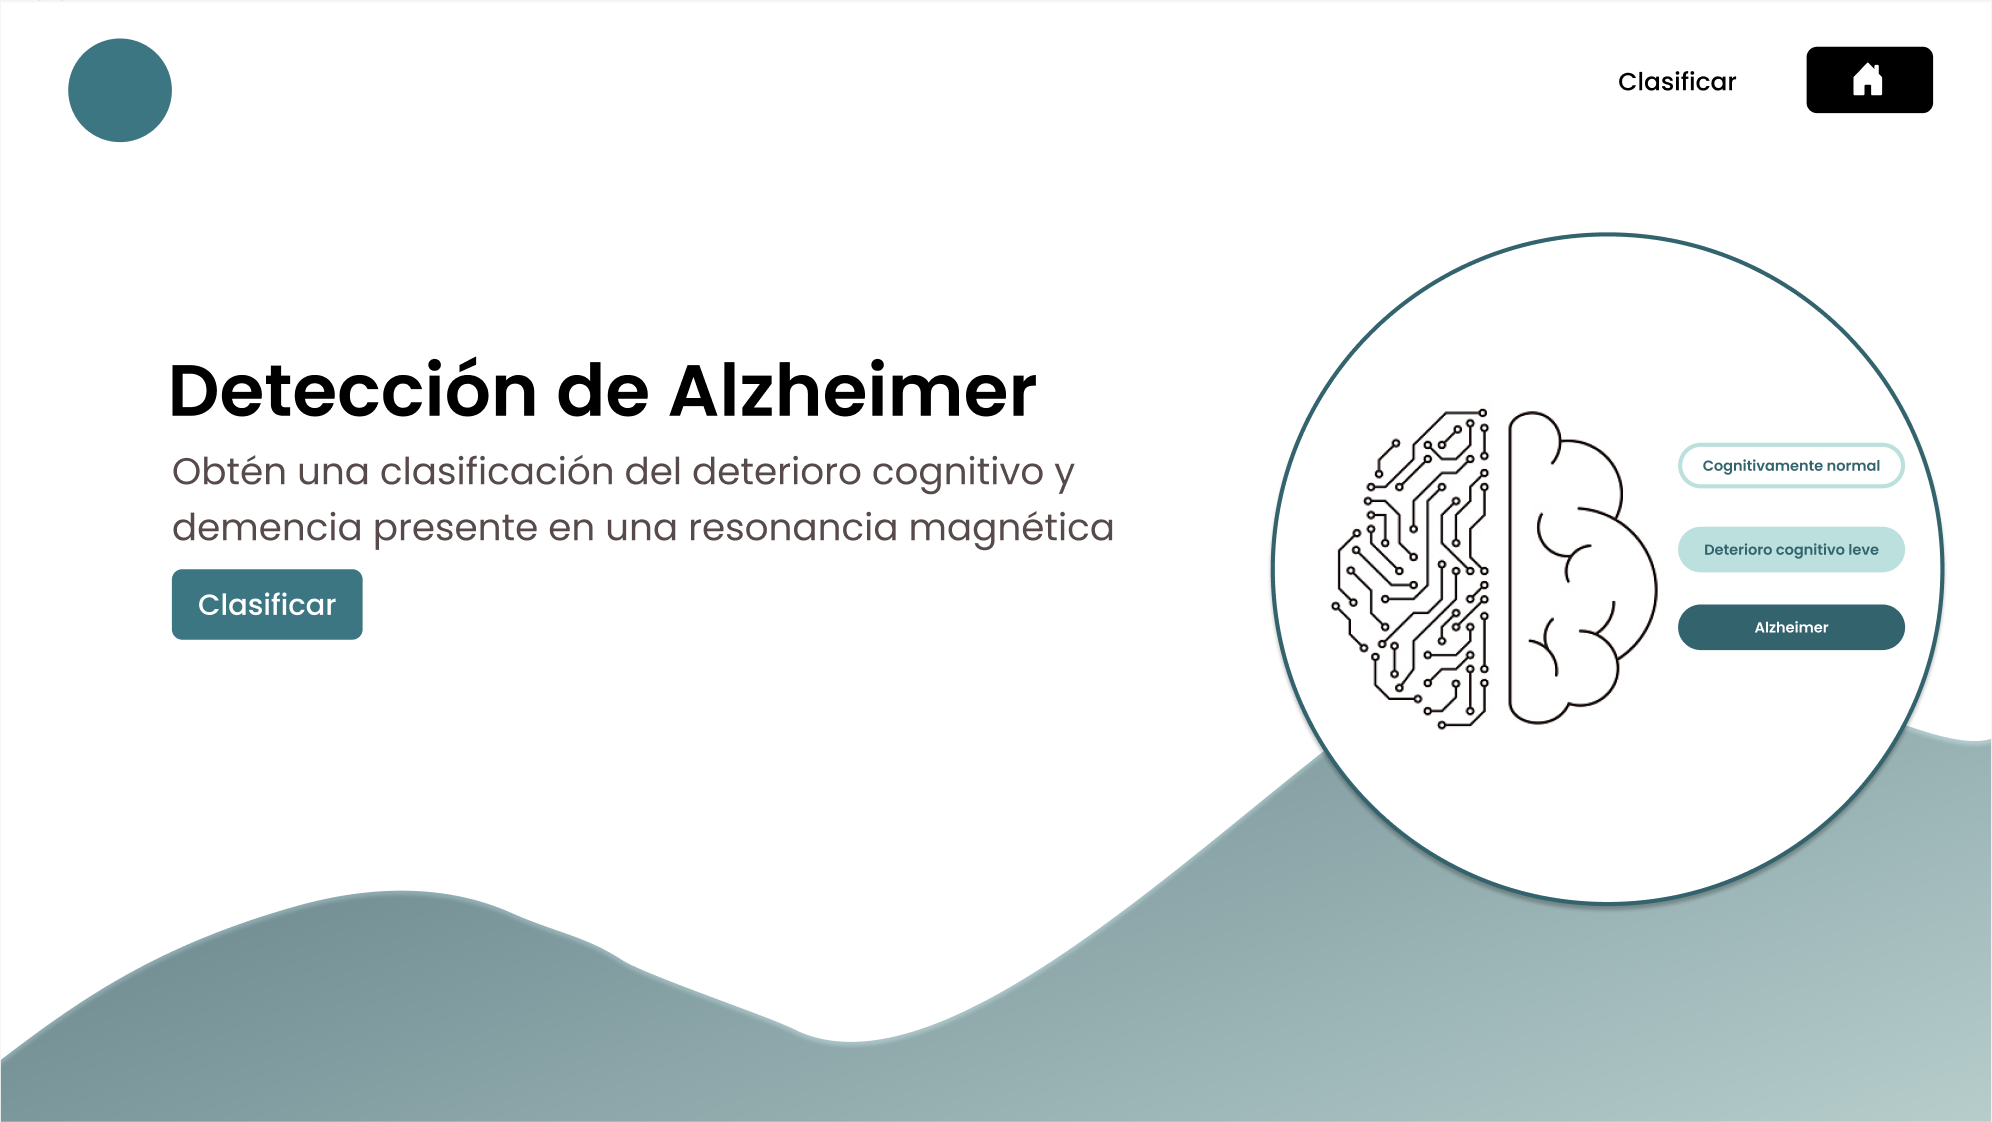
\includegraphics[width=\textwidth]{./imgs/app/landing-page}
    \caption{Landing Page}
    \label{fig:landing-page}
\end{figure}

\begin{figure}[H]
    \centering
    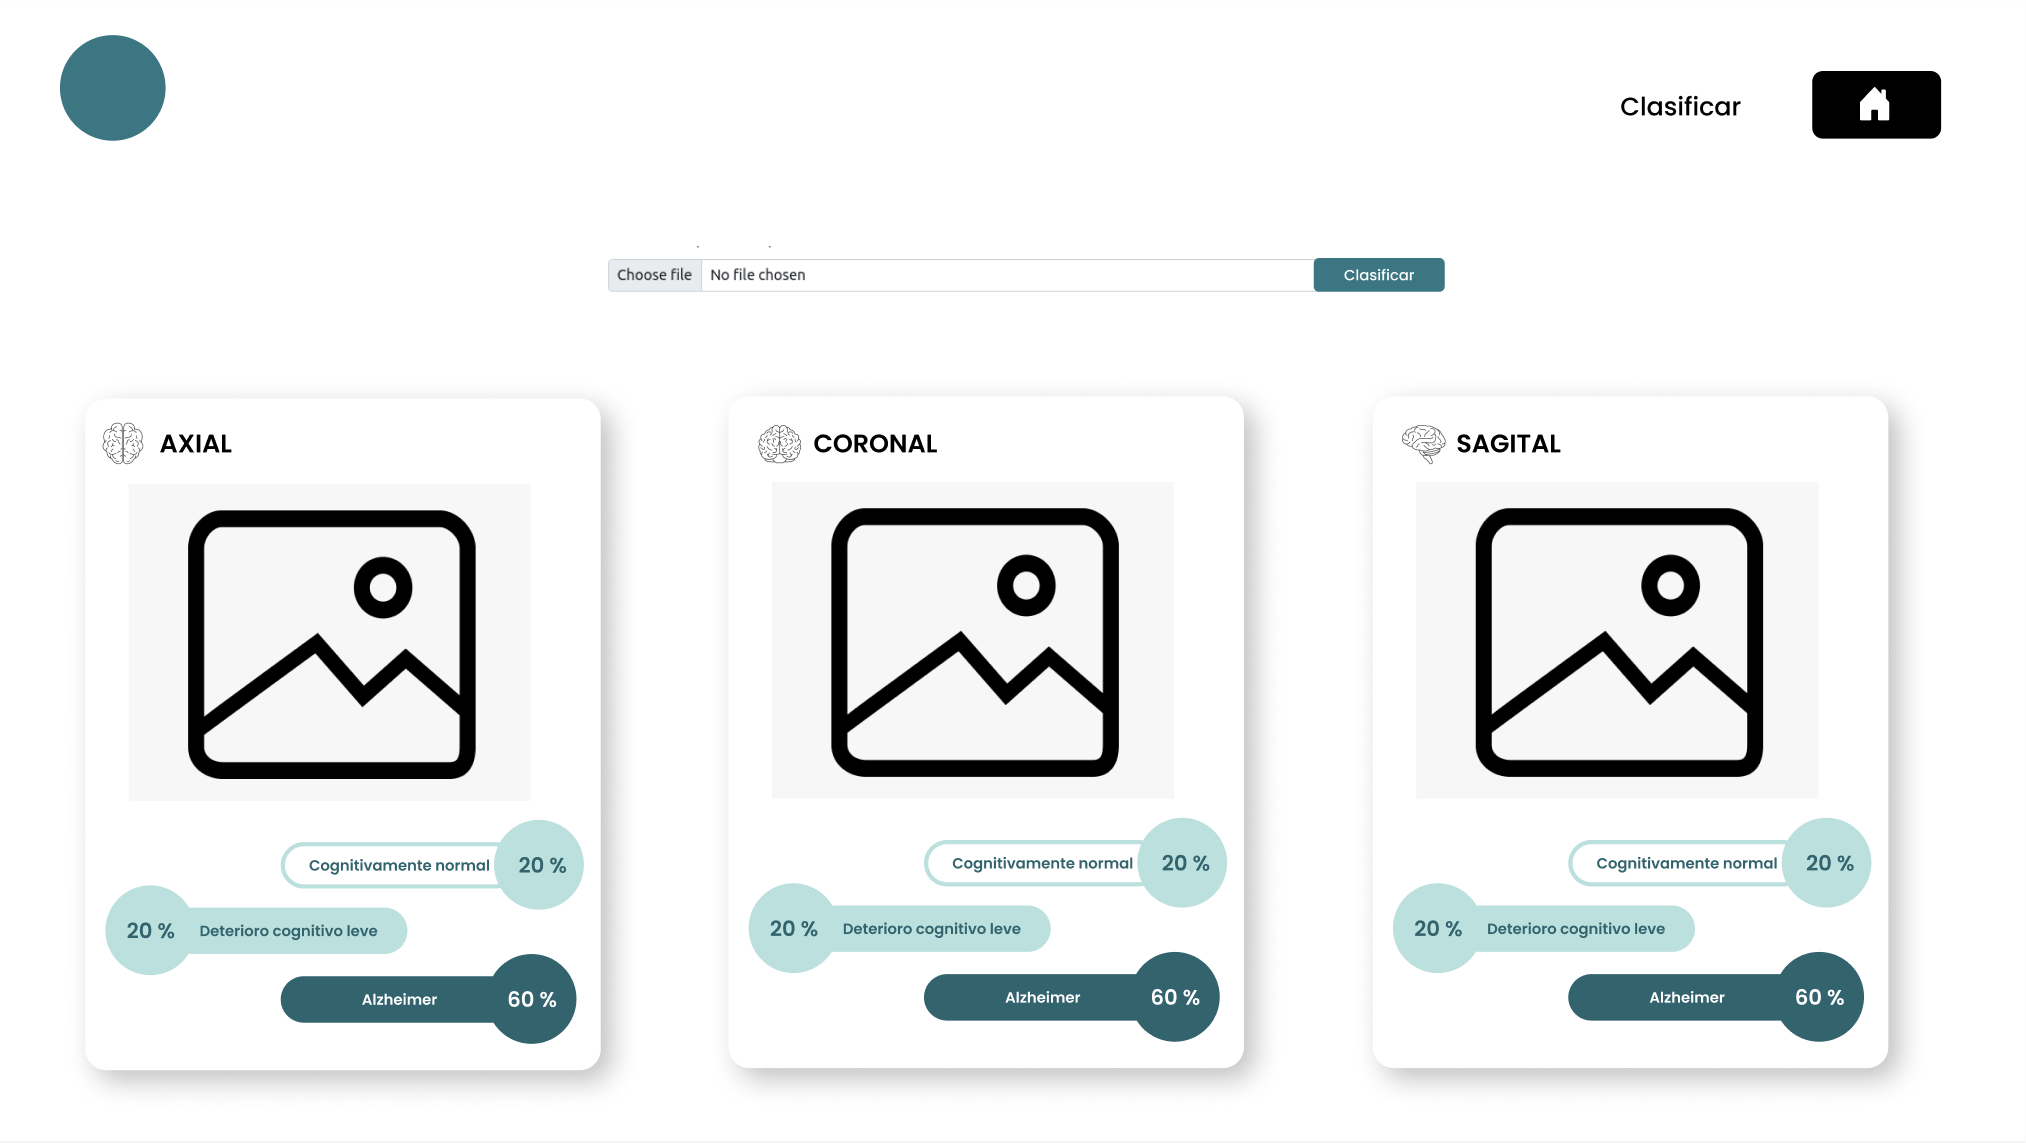
\includegraphics[width=\textwidth]{./imgs/app/vista-clasificacion}
    \caption{Vista De Clasificación}
    \label{fig:vista-clasificacion}
\end{figure}

\section{Implementación}\label{sec:implementacion}
Para la implementación de \textbf{Alz Care} se ha decidido usar una arquitectura
\textit{cliente-servidor}~\footnote{Modelo de comunicación \href{https://definicion.de/cliente-servidor/}{cliente-servidor}}, facilitando
así la utilización de la parte del servidor por otras aplicaciones o servicios de cara a posteriores trabajos.

En el lado del servidor o backend es donde se encuentra la lógica de la aplicación y donde se va a realizar la
integración con el sistema de aprendizaje profundo.
Se mantiene como lenguaje de programación Python, para poder seguir haciendo uso de las librerías necesarias para el
procesamiento de biomarcadores MRI de tipo NIfTI y las herramientas para trabajar con el sistema de DL.

Como framework se ha utilizado \textbf{flask-smorest}, una librería framework para crear API REST de la mano de
\textbf{Flask}, que es un genial candidato para desarrollar API en Python de manera ágil que dispone de un depurador
y soporte integrado para pruebas unitarias.
Además como herramienta de validación de datos se utiliza \textbf{marshmallow} y para la documentación de la API se utiliza
\textbf{Swagger}.

Para la gestión de dependencias se utiliza \textbf{Poetry}, ya que es una herramienta gestiona las bibliotecas de las que depende
tu proyecto por ti.
Evitando errores entre versiones y facilitando la creación del entorno de trabajo.

Del lado del cliente se ha utilizado \textbf{React} por ser una librería muy completa con la que crear interfaces de usuario
mediante componentes de manera sencilla.
Y que dispone de un amplio abanico de librerías externas, como \textbf{Framer Motion}, una biblioteca de animación que ha
facilitado la integración de animaciones mejorando la experiencia de usuario de la aplicación.

Como parte de la metodología de trabajo, se han incluido como Integración Continua dos pipelines para el código al
proyecto en \textit{GitHub} Actions para asegurar la integridad de la aplicación a la incorporación de nuevas funcionalidades.
Se ha incorporado uno para el backend y otro para el frontend, en ambos se persigue la misma meta: evitar errores en
el código fuente, mediante flake8 para el servidor y prettier para el frontend, y la ejecución de tests.


\section{Resultados}\label{sec:resultados}

\begin{figure}[H]
    \centering
    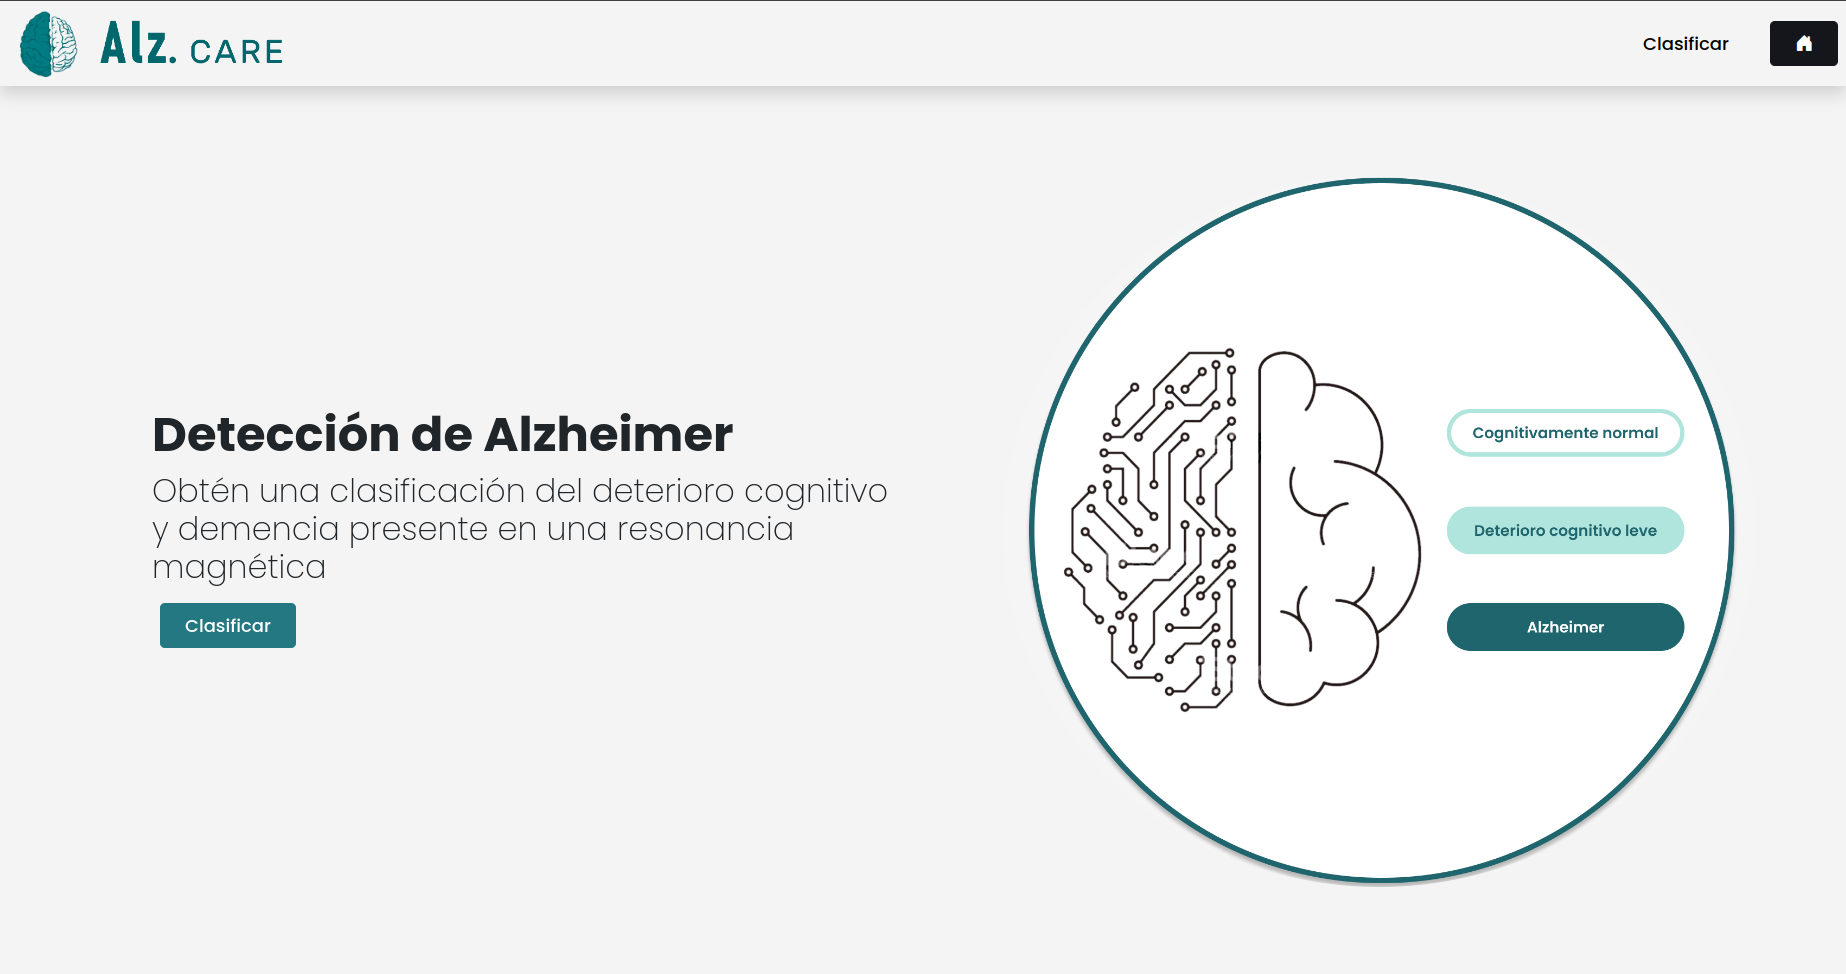
\includegraphics[width=\textwidth]{./imgs/app/final-home}
    \caption{Home Page de Alz Care}
    \label{fig:home-page}
\end{figure}

\begin{figure}[H]
    \centering
    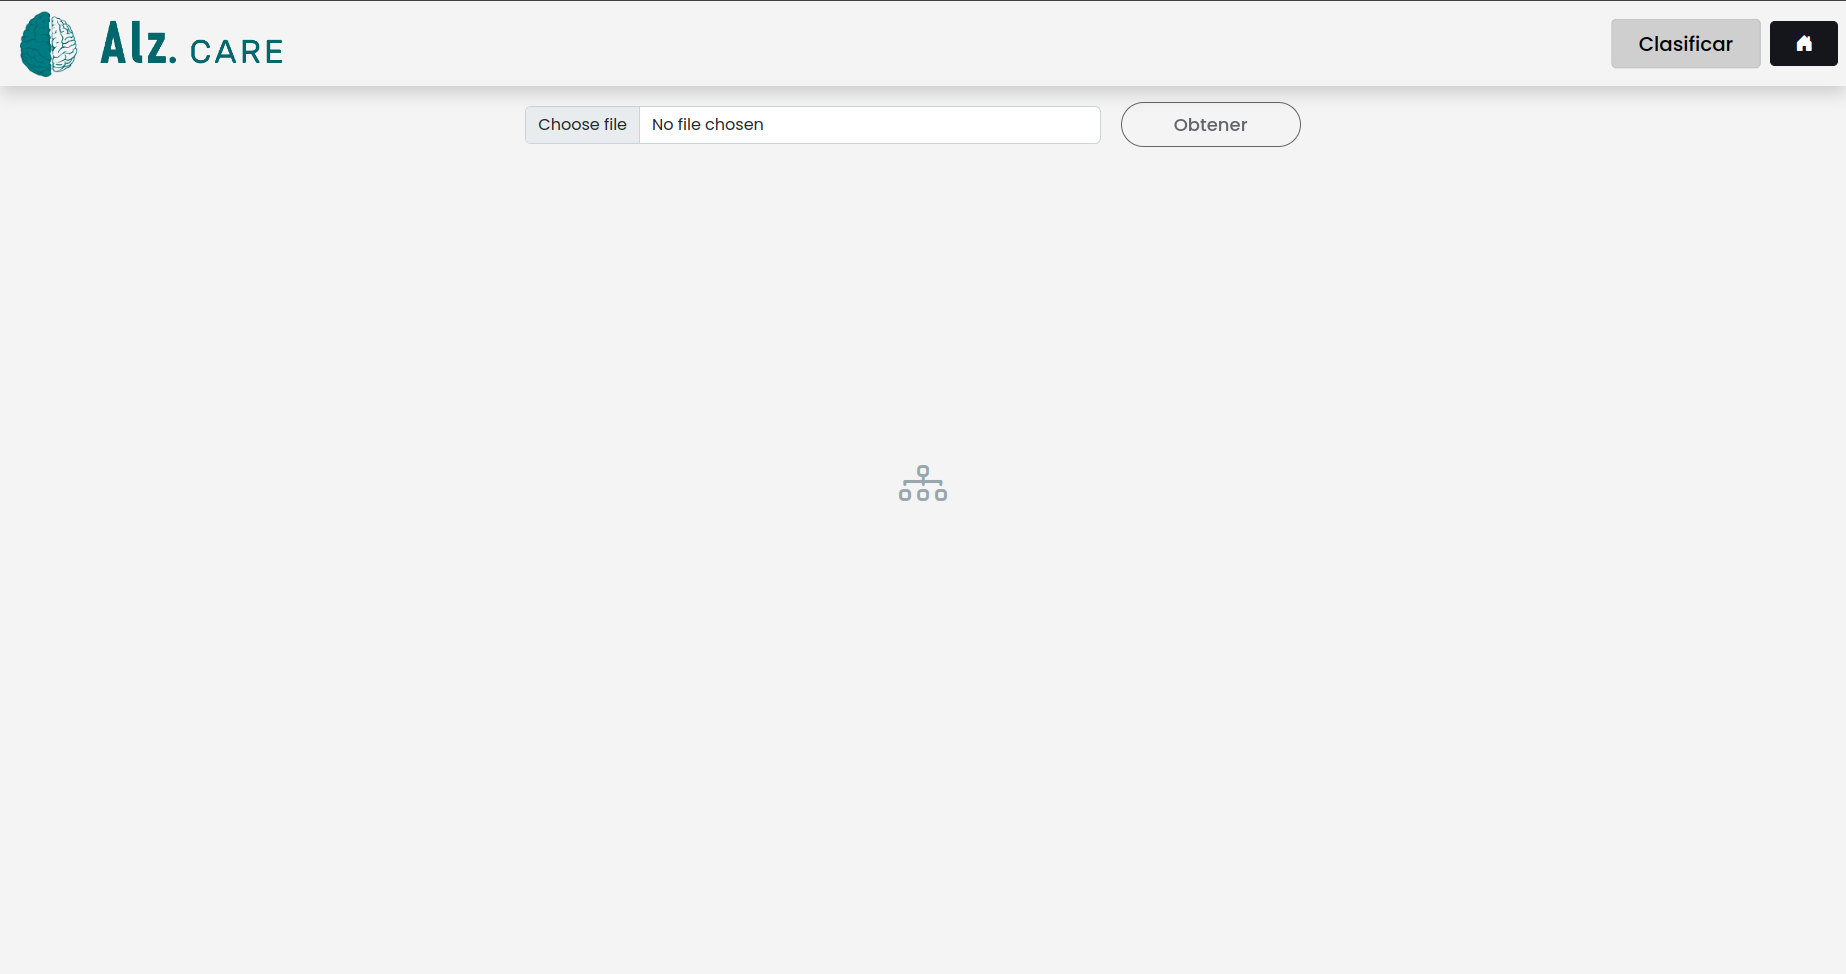
\includegraphics[width=\textwidth]{./imgs/app/final-cp}
    \caption{Vista De Clasificación de Alz Care}
    \label{fig:final-cp-page}
\end{figure}

\begin{figure}[H]
    \centering
    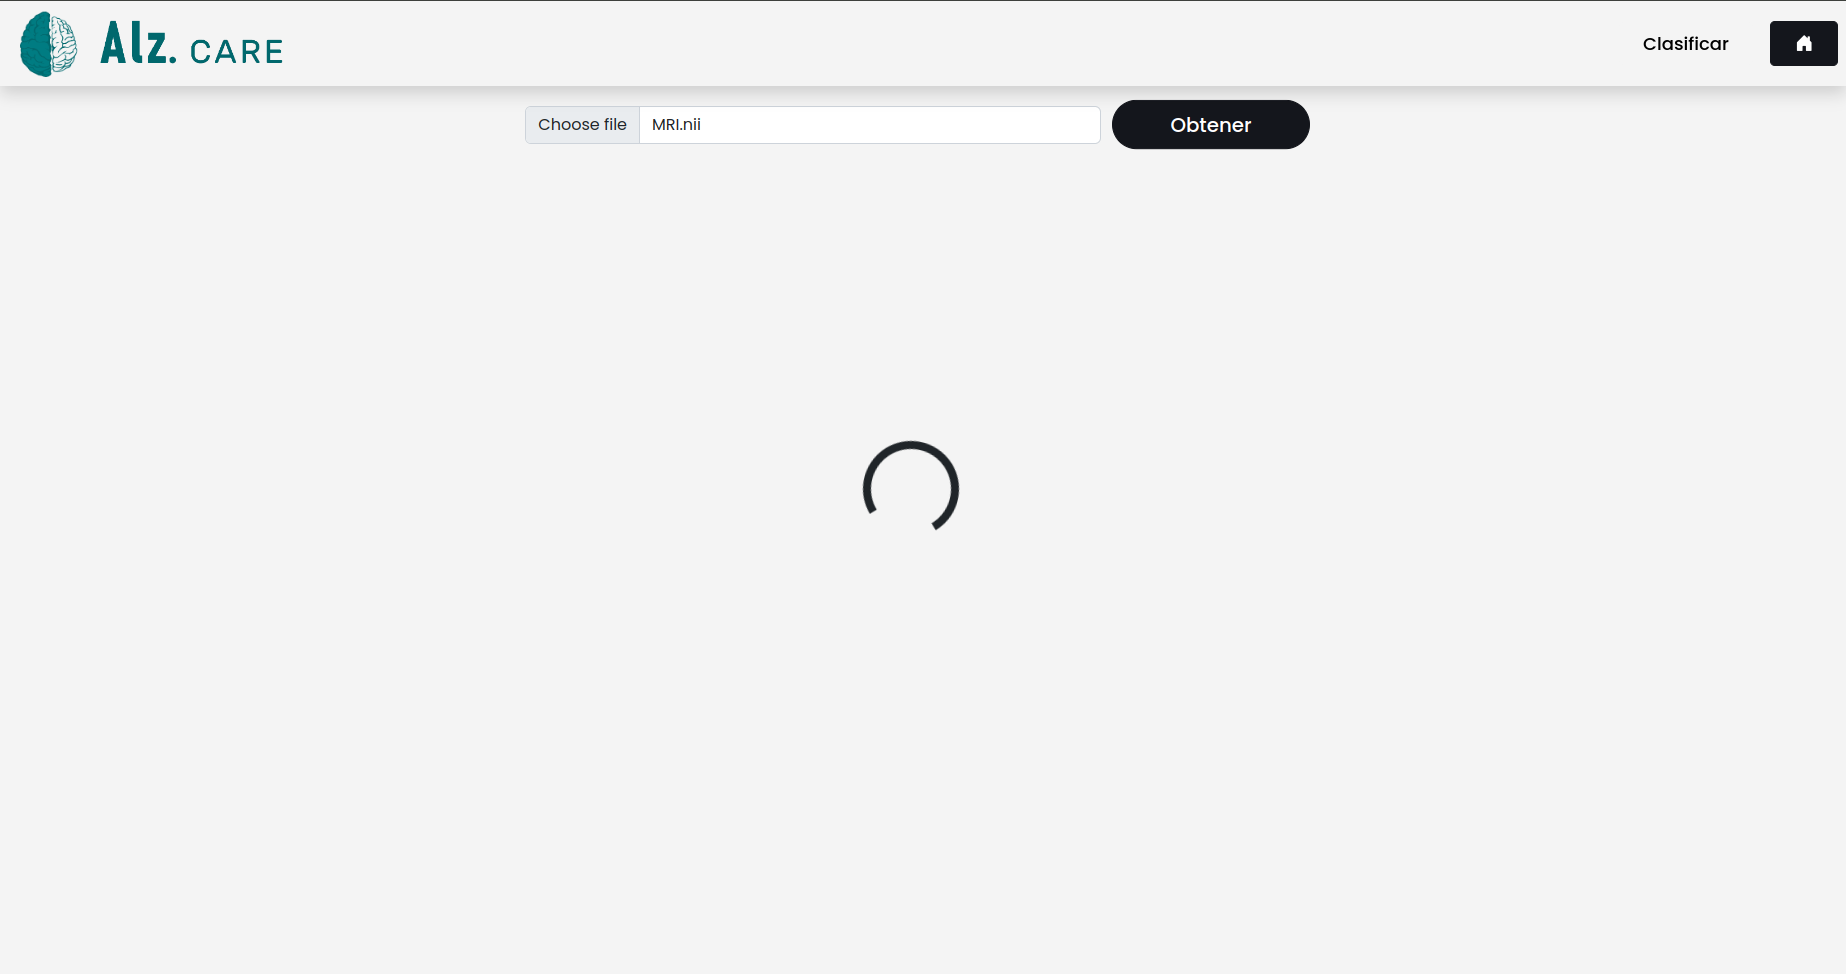
\includegraphics[width=\textwidth]{./imgs/app/final-cp-l}
    \caption{Vista De Clasificación de Alz Care: Cargando datos}
    \label{fig:final-cp-l-page}
\end{figure}

\begin{figure}[H]
    \centering
    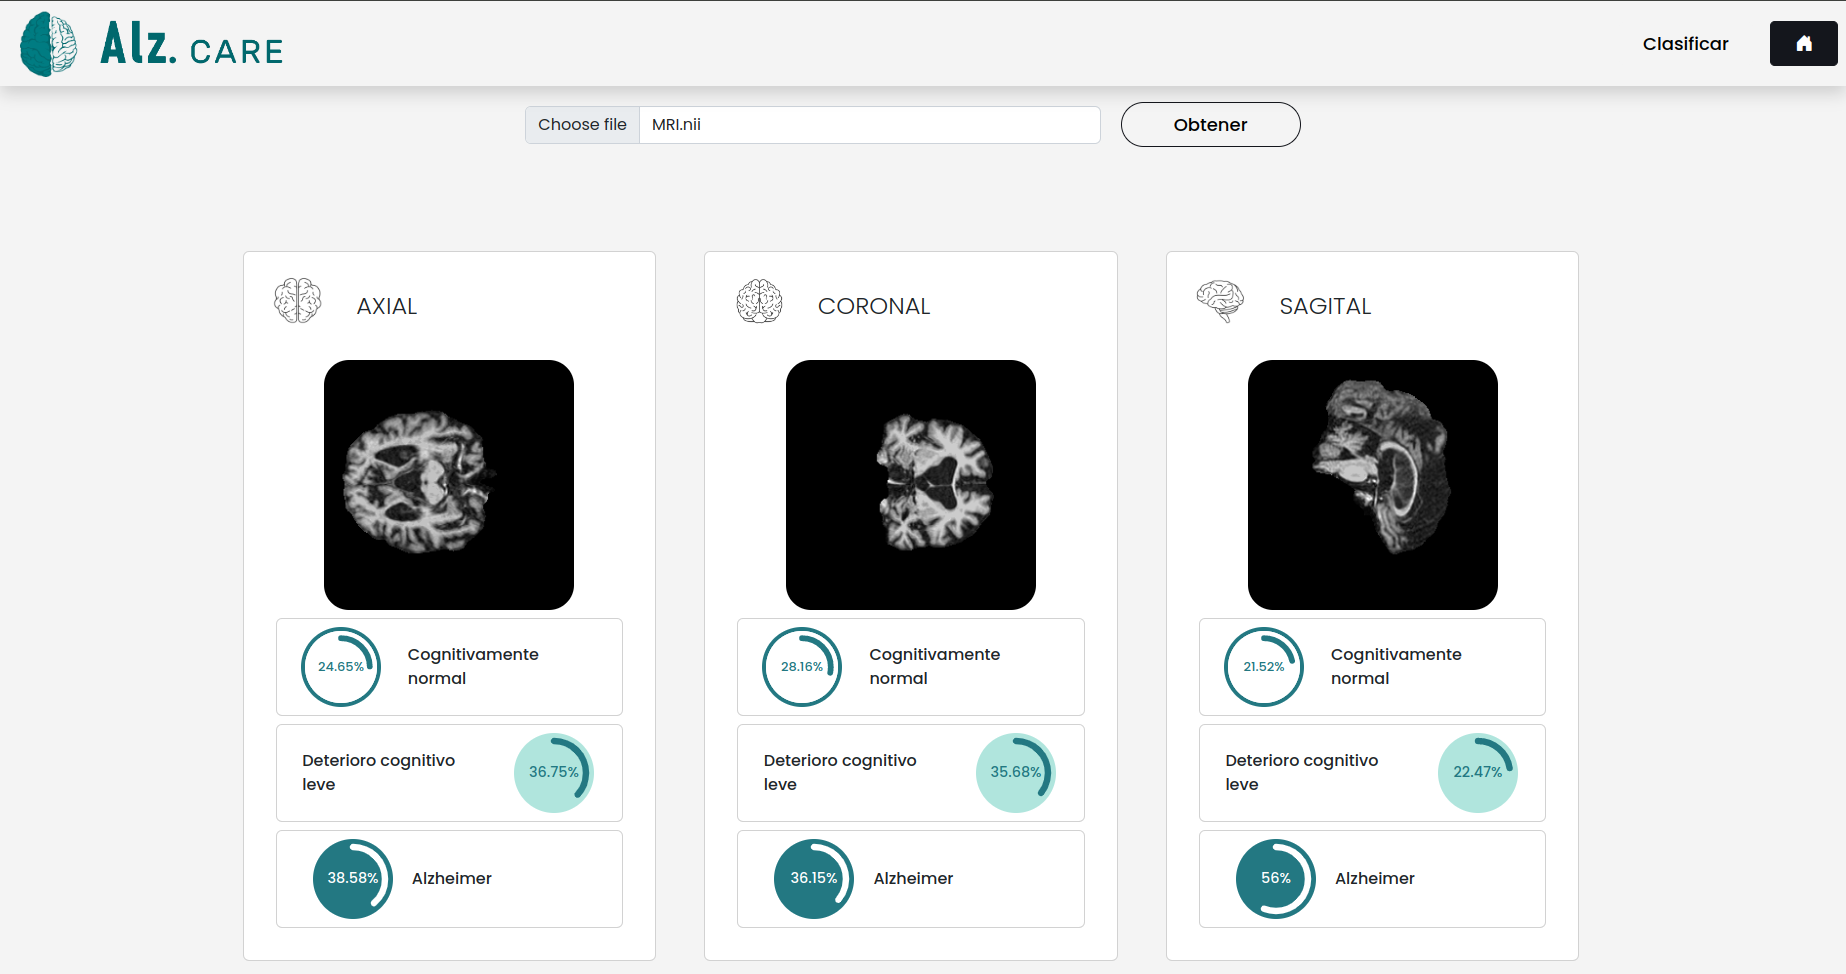
\includegraphics[width=\textwidth]{./imgs/app/final-cp-r}
    \caption{Vista De Clasificación de Alz Care: Resultados}
    \label{fig:final-cp-r-page}
\end{figure}